% Some classes load the `subfigure` package which clashes with
% our internal use of `subfig` for subfloats. We are most likely
% not going to need the canned subfigure functionality anyways,
% so we'll trick LaTeX into thinking it already loaded `subfigure`
\makeatletter
\newcommand{\dontusepackage}[2][]{%
  \@namedef{ver@#2.sty}{9999/12/31}%
  \@namedef{opt@#2.sty}{#1}}
\makeatother
\dontusepackage{subfigure}


%% ===== Begin LaTeX file ===========================
%%
\documentclass[]{article}

\usepackage{lmodern}
\usepackage{amssymb,amsmath}
\usepackage{ifxetex,ifluatex}
\usepackage[usenames,dvipsnames]{color}
\usepackage{fixltx2e} % provides \textsubscript
\ifnum 0\ifxetex 1\fi\ifluatex 1\fi=0 % if pdftex
  \usepackage[T1]{fontenc}
  \usepackage[utf8]{inputenc}
\else % if luatex or xelatex
  \ifxetex
    \usepackage{mathspec}
    \usepackage{xltxtra,xunicode}
  \else
    \usepackage{fontspec}
  \fi
  \defaultfontfeatures{Mapping=tex-text,Scale=MatchLowercase}
  \newcommand{\euro}{€}
\fi
% use upquote if available, for straight quotes in verbatim environments
\IfFileExists{upquote.sty}{\usepackage{upquote}}{}
% use microtype if available
\IfFileExists{microtype.sty}{%
\usepackage{microtype}
\UseMicrotypeSet[protrusion]{basicmath} % disable protrusion for tt fonts
}{}
\usepackage{listings}
% Define slightly more reasonable Listings defaults
\lstset{
    basicstyle=\ttfamily\small,
    breaklines=true,
    prebreak=\raisebox{0ex}[0ex][0ex]{\ensuremath{\hookleftarrow}},
    frame=lines,
    showtabs=false,
    showspaces=false,
    showstringspaces=false,
    keywordstyle=\color[gray]{0.4}\bfseries,
    commentstyle=\color[gray]{0.65}\itshape,
    numbers=left,
    captionpos=b,
}
\usepackage{longtable,booktabs}
\usepackage{graphicx}
\makeatletter
\def\maxwidth{\ifdim\Gin@nat@width>\linewidth\linewidth\else\Gin@nat@width\fi}
\def\maxheight{\ifdim\Gin@nat@height>\textheight\textheight\else\Gin@nat@height\fi}
\makeatother
% Scale images if necessary, so that they will not overflow the page
% margins by default, and it is still possible to overwrite the defaults
% using explicit options in \includegraphics[width, height, ...]{}
\setkeys{Gin}{width=\maxwidth,height=\maxheight,keepaspectratio}
\usepackage{caption}
\usepackage{float}
% Override extremely conservative LaTeX float placement rules
% (might need to be removed for "manuscript" styles)
\renewcommand{\topfraction}{0.85}	% max fraction of floats at top
\renewcommand{\bottomfraction}{0.75}	% max fraction of floats at bottom
\setcounter{topnumber}{2}
\setcounter{bottomnumber}{2}
\setcounter{totalnumber}{4}
\setcounter{dbltopnumber}{2}    % for 2-column pages
\renewcommand{\dbltopfraction}{0.85}	% fit big float above 2-col. text
\renewcommand{\textfraction}{0.10}	% allow minimal text w. figs
\renewcommand{\floatpagefraction}{0.85}	% require fuller float pages
\renewcommand{\dblfloatpagefraction}{0.85}	% require fuller float pages
% Encourage floats to be placed in the vacinity of where it is defined
% (in some manuscript styles where figures are collected at the end, the 'h'
% option might need to be removed by a separate '\floatplacement' call in the
% 'header-includes' metadata field)
\floatplacement{figure}{htbp}
\floatplacement{scholmdAlgorithm}{htbp}
\floatplacement{table}{htbp}
\ifxetex
  \usepackage[setpagesize=false, % page size defined by xetex
              unicode=false, % unicode breaks when used with xetex
              xetex]{hyperref}
\else
  \usepackage[unicode=true]{hyperref}
\fi
\hypersetup{breaklinks=true,
            bookmarks=true,
            pdfauthor={Neal van Veen},
            pdftitle={A better webcrawler in Go},
            colorlinks=true,
            citecolor=black,
            urlcolor=blue,
            linkcolor=black,
            pdfborder={0 0 0}}
\urlstyle{same}  % don't use monospace font for urls
\setlength{\parindent}{0pt}
\setlength{\parskip}{6pt plus 2pt minus 1pt}
\setlength{\emergencystretch}{3em}  % prevent overfull lines
\setcounter{secnumdepth}{5}


\title{A better webcrawler in Go\\\vspace{0.5em}{\large Multimedia Information Retrieval}}
\author{Neal van Veen}
\date{\today}

\usepackage{cleveref}


\begin{document}
\maketitle
\begin{abstract}
The Go programming language by Google is a new and modern
statically-typed, compiled language designed to aid developers in
creating large applications, with fast compilation times, modern
concurrency primitives, simple syntactical elements and a large standard
library. Webcrawlers are programs that delve into the sources of
webpages and index certain elements to be used for querying at a later
time by a consumer. This crawling is highly parallelizable, so we
examine the creation of a webcrawler written in Go and test its various
concurrency features, alongside two datastructures that show how
programming in Go works. Results show a marked improvement over
sequential crawling, hitting a performance ceiling at about 100
goroutines. We then conclude the goal of this project was succesful. The
code for this project can be found at
\url{https://github.com/Nvveen/mir}, and all source code was written by
the author.
\end{abstract}

\section{Introduction}\label{introduction}

\subsection{Go}\label{go}

The Go programming language was created by Robert Griesemer, Rob Pike
and Ken Thompson (the latter two of C-fame). The language specification
was drafted in 2007, and the first release was in 2009, and the language
achieved stability with the 1.0-release in 2012. Its syntax was loosely
inspired by C, and it is very reminiscent in its simplicity. However, Go
is created to be much more type-safe, and to provide far more modern
tools to add the developer, as such tooling is needed when dealing with
the large-scale applications that are made at Google. From its
inception, Go has been an open-source project, and since 2015 is
maintained at \href{https://github.com/golang}{Github}.

\subsection{Features}\label{features}

Go has adopted a range of patterns from dynamic programming languages,
like type inference with the \texttt{:=} declaration operator. To
determine a type beforehand, a user can also declare like this:
\texttt{var i int}. Go was also created for extremely fast compilation
times, to aid in rapid development and deployment. Indeed, oftentimes
compiling and running a Go script is faster than simply interpreting a
similar script in Python.

A range of tools exist that help development management in the Go
ecosystem. Package managment is done by the \texttt{go} tool, so that
dependency management issues are minimalized. If a dependency is
specified in the source code, the programmer only has to run
\texttt{go get} to retrieve, or \texttt{go get github.com/Nvveen/mir} to
retrieve another package. Installing a retrieved package puts a
package's binary in the \texttt{pkg/bin/} directory in the location
specified by the environment variable \texttt{GOPATH}. This is done to
isolate packages.

The compiler is very strict when not using variables or modules, and
will throw an error if this happens. In the same way, certain writing
styles are prohibited, like putting an opening accolade \texttt{\{} on
the next line after an \texttt{if}-statement, because Go infers the
place of a semicolon statement terminator. These strict rules are also
implemented to allow the \texttt{go} tool to format source code along
these lines, having users run the \texttt{go fmt} tool to ensure all
source looks the same, improving readability. Exports of functions and
structures are done via capitalization. Each element that starts with a
capital letter can be accessed by other packages (assuming the package
itself is a library). As such, these functions' documentation are given
to the documentation generator.

Certain rules also exist for unit-testing. Each package can have
multiple source files in the same directory, all ending with
\texttt{.go}. However, if a file ends with \texttt{\_test.go}, the
\texttt{go test} tool will run all testing functions in these files
starting with \texttt{TestXXX}, and a certain function signature. Other
functions in these files that are accepted are \texttt{BenchmarkXXX} and
\texttt{ExampleXXX} functions, where benchmarking allows you to test the
performance of certain parts of the package. Example-functions are
functions that can be added to automatically generated documentation of
the source code (see next paragraph).

Documenting the source is very easy in Go. \texttt{package} declarations
are the first syntatical elements that name a package. However, any
comments starting with \texttt{//} preceding this line is assumed to be
package-wide text explaining what the package does. Comments preceding
function declarations are assumed to be documentation of these
functions, and depending on whether these functions are exported,
documentation is generated with the \texttt{go doc} tool. This tool can
create a local HTTP-server for a user to view the code documentation, or
other output formats are generated, such as plain text. Examples in
unit-testing code are also added to the documentation pages in the
server, and can actually be run in many instances.

Go compiles all of its code almost exclusively statically, which means
deployment to other machines and architectures (the compiler supports
cross-compiling) is very easy and a deployer doens't have to worry about
dependency issues. Version management is done by simpy recompiling, as
the compiler is fast enough to not make this a hassle.

Concurrency is the way in which modern languages can distinguish
themselves from older languages. Go's concurrency primitives support
communicating sequential processes, by having primitives such as
channels, selection from these channels and light-weight processes
called \texttt{goroutines}. Each function can be started in a new
goroutine simply by preprending \texttt{go} to the function call.

Go does not support inheritance or true objects, but rather the C way of
defining structures with \texttt{struct} (\texttt{type Foo struct \{\}})
and supplementing it with interfaces, so duck-typing can be used
(\texttt{type Bar interface\{\}}). Each object that implements the
functions in an interface is implicitly assumed to implement this
interface too, allowing for a lot of generalizability.

From the start, Go has enjoyed a large standard library, with a big set
of features, such as packages to implement webservers, compression
algorithms, text parsing, and much more. In this project, most of the
external packages are from this standard library.

For better or for worse, Go does away with a lot of language elements
that have been at the forefront of programming for decades. Go does not
support generics, assertions, operator overloading, inheritance (only
embedding of types), or \texttt{const} specifiers. Type assertions also
allow a programmer to circumvent Go's type system rather easily. Go also
uses a garbage collector, and pointer arithmetic does not exist in the
language. As such, the GC does bring an overhead and Go does need a
runtime to properly work. Other modern elements are present, such as
slices, hashmaps.

\subsection{Webcrawler}\label{webcrawler}

A webcrawler is a type of program that typically runs on systems with
large infrastructures to systematically crawl (or index) links on pages,
and parse the resulting new pages for new links, words and other
metadata associated with the contents of the file. For this reason, most
webcrawlers are not really suited for semantic searching, as no actual
content is reasoned about yet by most webcrawlers. As such, these
operations of indexing are fairly basic. However, because each page can
be indexed separately, these operations are highly parallelizable, both
on the link level, and on the page level. For this assignment, we will
examine the parallelization on the link level, although the code can be
easily extended to support concurrent indexing on the page level.

\begin{figure}
\centering
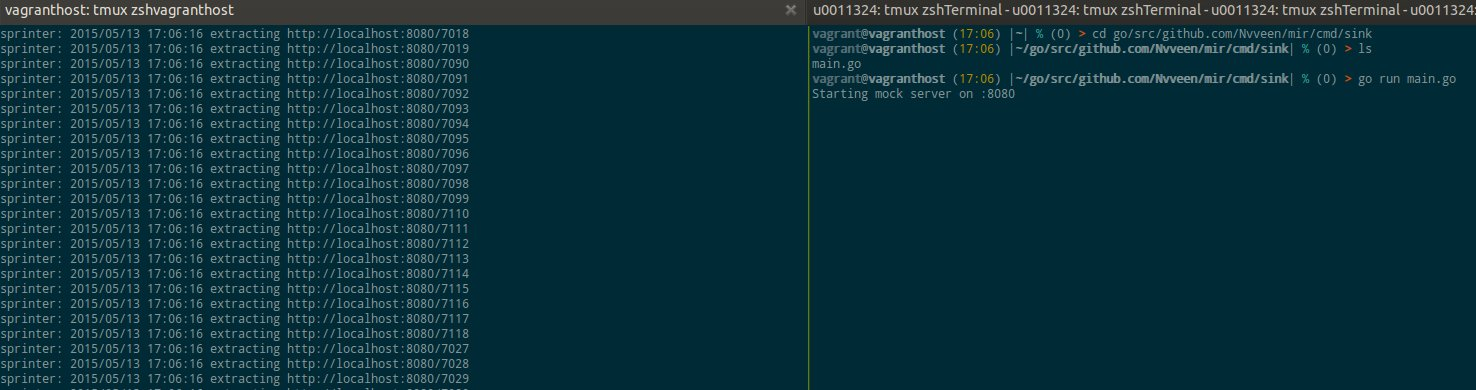
\includegraphics[]{img/screen.jpg}
\caption{An example of output.}\label{figexample}
\end{figure}

\section{Research Description}\label{research-description}

The features mentioned in Section \ref{features} are used to create a
webcrawler in Go and determine its suitability for this specific kind of
task. We will also determine its performance in a sequential manner
compared to a concurrent crawl. There is three main packages in the
source code, called \texttt{sprinter}, \texttt{storage}, and
\texttt{container}. \texttt{storage.go} and \texttt{container.go}
contain interfaces defining the types that are used in the crawler. This
is done for modularity, and supporting different types of containers or
storage is trivial to implement. In fact, the main storage type uses a
MongoDB-backend, although unit-testing code reimplements the interface
for a simple hashmap, as the testing is done exclusively on the crawler
code, and testing for the container is done in its own testing package.

Even in sequential mode, the crawler uses a channel with the size of the
maximum amount of concurrent requests (or in this case just the one
request). The first goroutine queries this channel and retrieves a link
from it, after which a function is launched (in the same goroutine if
sequential). Because a new goroutine is launched in concurrent mode,
this function call is non-blocking, and consequently, a number of
concurrent requests can be done, depending on the
\texttt{MaxConcurrentRequests} variable that can be changed depending on
the need.

The crawler uses the storage-backend to store its indexing results such
as words in the title and page and checksums of links on a page. A
container is used to store visited links, while another hashmap is used
to store query results for a host's \texttt{robots.txt}, so we don't
visit pages we aren't supposed to visit. Simple control statements are
used to clean this hashmap every two thousand links, because we need to
revisit every once in a while. The container mainly helps in checking
for duplicates, and currently two types are implemented: a linked list
and a binary search tree. Future work can be done in implementing a
\texttt{fragment tree}, a type of tree data structure which uses
fragments of a URI, such as the subdomain, host, and path as keys in the
tree, to quickly search and minimize the size of the data structure when
storing links. As mentioned, \texttt{robots.txt} is also parsed, using
one of the few external libraries.

Each function written is immediately documented and unit-tests are
written before each function is implemented, to ensure coverage of the
code. This approach, however, did necessitate a few different things. To
test the webcrawler on a set of pages, we decided against actual net
crawling. Because of this, a small sink program was created that
generated a page on the localhost's root, with a set of links pointing
to more pages on the localhost, that were automatically generated. Each
request was delayed with a 20ms delay, as to simulate actual requests.
To unit-test the storage backend for MongoDB, special scripts and code
was written to start a local MongoDB backend with the
\texttt{supervisor} program, which will destroy the unit-testing
database after completion. No experiments were run with a MongoDB
container on a different system in a network. Most unit-tests with the
crawler used a mock storage object, which was nothing more than a
hashmap that implemented the same interface that MongoDB does.

\section{Experiments}\label{experiments}

The language features mentioned in Section \ref{features} also contain
benchmarking functionality alongside the unit-testing functionality.
This set of features was used to determine efficiency and speed of
crawling.

Sets of 1, 10, 50, 100, 500, and 1000 concurrent requests are tested 5
times each and averaged. These sets use a static list as a container,
and a mock storage as backend. Each crawl stops after 2000 total
requests performed. See figures \ref{fig2} and \ref{fig3}, and figure
\ref{fig6} for the number of allocations done.

\begin{figure}
\centering
\includegraphics[]{plots/1.eps}
\caption{Concurrent crawling.}\label{fig2}
\end{figure}

\begin{figure}
\centering
\includegraphics[]{plots/2.eps}
\caption{Concurrent crawling up to 100 goroutines.}\label{fig3}
\end{figure}

\begin{figure}
\centering
\includegraphics[]{plots/1_alloc.eps}
\caption{Concurrent crawling up to 100 goroutines and its
allocations.}\label{fig6}
\end{figure}

Then, sequential crawling is done for a static list and a binary search
tree as containers. See figure \ref{fig1}.

\begin{figure}
\centering
\includegraphics[]{plots/sequential.eps}
\caption{Sequential crawling allocations.}\label{fig1}
\end{figure}

More than 100 requests don't show a significant boost in execution time,
so this number of requests is also done to test the performance gains
for a MongoDB backend, a binary search tree container, and both. See
figure \ref{fig4}.

\begin{figure}
\centering
\includegraphics[]{plots/bar.eps}
\caption{MongoDB and Binary Search Tree comparisons.}\label{fig4}
\end{figure}

As can be seen, processing with a MongoDB backend takes longer, as this
data needs to be inserted into the database, which takes longer than for
an in-memory data structure. The other way in which they differ is in
the amount of allocations, as can be seen in figure \ref{fig5}.

\begin{figure}
\centering
\includegraphics[]{plots/alloc.eps}
\caption{MongoDB and Binary Search Tree allocations
comparisons.}\label{fig5}
\end{figure}

\begin{table}
\centering
\begin{tabular}{llllll}
\toprule\addlinespace
Concurrent Requests & ms/operation & s/operation & B/operation & Storage
& Container\tabularnewline
\midrule
1 & 406314 & 406 & 2183831 & Static & List\tabularnewline
10 & 42379.8 & 42 & 155034526 & Static & List\tabularnewline
50 & 12000.6 & 12 & 169152106 & Static & List\tabularnewline
100 & 6793.2 & 7 & 175794790 & Static & List\tabularnewline
500 & 5548.2 & 6 & 180991330 & Static & List\tabularnewline
1000 & 5517 & 6 & 186980419 & Static & List\tabularnewline
100 & 5837.8 & 6 & 172357893 & Static & BST\tabularnewline
100 & 168390.2 & 168 & 350009446 & MongoDB & List\tabularnewline
100 & 70705.8 & 71 & 335336514 & MongoDB & BST\tabularnewline
1 & 406316.4 & 406 & 154093070 & Static & BST\tabularnewline
\bottomrule
\end{tabular}
\caption{A summary of the data.}\label{table1}
\end{table}

\section{Discussion}\label{discussion}

The results clearly show a huge improvement in crawling speed, of about
10\% of a sequential crawl for 2000 requests. This isn't strange, and
the same results (or even better), can probably be obtained using
another programming language and concurrency primitives. However, the
goal of this project was to determine how to do it in Go, so these
results provide a validation alongside the fact that significant gains
can be made just by parallelizing the tasks. Another advantage to Go is
the usage of the standard library in writing an entire crawler, as these
codebases tend to be idiomatic and highly scrutinized for (code
quality), and as such, can be assumed to be `correct'. The biggest
reason for picking Go personally, was its focus on making concurrent
programming accessible, and while we did run into problems, the language
itself made us much more comfortable in trying to accomplish the
assignment. These problems were, after all, more related with the
difficulties inherent to concurrent programming, such as synchronization
and buffering. Once these hurdles were taken, Go only helped in creating
a highly performant webcrawler.

Other points that can be made from the results, is that using a binary
search tree also offers clear advantages, and the combination of about
100+ goroutines and a binary search tree as a container pushed our 2000
request-crawl under 6 seconds.

However, using a MongoDB database did slow the program down a bit.
However, the indexing results had to be stored on disk, which is always
slower than in memory, what the static list was doing, and which is an
approach unsuitable for actual crawling in real time on a server or
cluster.

\section{Conclusions}\label{conclusions}

Picking Go was a decision based on prior knowledge of the language, and
the fact that the reasons Go was created seemed to be in line with the
requirements for a webcrawler. It was only natural to create a
webcrawler using Go's modern language elements, and analyze its
performance. The results show that this decision was not the wrong one,
and significant gains can be made, while avoiding pitfalls commonly
associated with other programming languages, such as language complexity
and ambiguity.


\end{document}

